\documentclass[
	a4paper
]{scrreprt}

%%% PACKAGES %%%

% add unicode support and use german as language
\usepackage[utf8]{inputenc}
\usepackage[ngerman]{babel}

% Use Helvetica as font
\usepackage[scaled]{helvet}
\renewcommand\familydefault{\sfdefault}
\usepackage[T1]{fontenc}

% Better tables
\usepackage{tabularx}

% Better enumerisation env
\usepackage{enumitem}

% Use graphics
\usepackage{graphicx}

% Have subfigures and captions
\usepackage{subcaption}

% Be able to include PDFs in the file
\usepackage{pdfpages}

% Have custom abstract heading
\usepackage{abstract}

% Need a list of equation
\usepackage{tocloft}
\usepackage{ragged2e}

% Better equation environment
\usepackage{amsmath}

% Symbols for most SI units
\usepackage{siunitx}

\usepackage{csquotes}

% Clickable Links to Websites and chapters
\usepackage{hyperref}

% Change page rotation
\usepackage{pdflscape}

% Symbols like checkmark
\usepackage{amssymb}
\usepackage{pifont}

\usepackage[absolute]{textpos}

% Glossary, hyperref, babel, polyglossia, inputenc, fontenc must be loaded before this package if they are used
\usepackage{glossaries}
% Redefine the quote charachter as we are using ngerman
\GlsSetQuote{+}
% Define the usage of an acronym, Abbreviation (Abbr.), next usage: The Abbr. of ...
\setacronymstyle{long-short}

% Bibliography & citing
\usepackage[
	backend=biber,
	style=apa,
	bibstyle=apa,
	citestyle=apa,
	sortlocale=de_DE
	]{biblatex}
\addbibresource{Referenzen.bib}
\DeclareLanguageMapping{ngerman}{ngerman-apa}

%%% COMMAND REBINDINGS %%%
\newcommand{\tabitem}{~~\llap{\textbullet}~~}
\newcommand{\xmark}{\ding{55}}

% Define list of equations - Thanks to Charles Clayton: https://tex.stackexchange.com/a/354096
\newcommand{\listequationsname}{\huge{Formelverzeichnis}}
\newlistof{myequations}{equ}{\listequationsname}
\newcommand{\myequations}[1]{
	\addcontentsline{equ}{myequations}{\protect\numberline{\theequation}#1}
}
\setlength{\cftmyequationsnumwidth}{2.3em}
\setlength{\cftmyequationsindent}{1.5em}

% Usage {equation}{caption}{label}
% \indexequation{b = \frac{\pi}{\SI{180}{\degree}}\cdot\beta\cdot 6378.137}{Bogenlänge $b$ des Winkels $\beta$ mit Radius 6378.137m (Distanz zum Erdmittelpunkt am Äquator)}{Bogenlaenge}
\newcommand{\indexequation}[3]{
	\begin{align} \label{#3} \ensuremath{\boxed{#1}} \end{align}
	\myequations{#3} \centering \small \textit{#2} \normalsize \justify }

% Todolist - credit to https://tex.stackexchange.com/questions/247681/how-to-create-checkbox-todo-list
\newlist{todolist}{itemize}{1}
\setlist[todolist]{label=$\square$}

%%% PATH DEFINITIONS %%%
% Define the path were images are found
\graphicspath{{./img/}{./pdf/}}

%%% GLOSSARY ENTRIES %%%
\makeglossaries
\newacronym{RFID}{RFID}{Radio-Frequency Identification}
\newglossaryentry{HF}{name={HF},description={High Frequency, RFID Tags im Frequenzbereich von 3-30MHz}}
\newglossaryentry{UHF}{name={UHF},description={Ultra High Frequency, RFID Tags im Frequenzbereich von 0.3-30GHz}}

%%% DOCUMENT %%%

\begin{document}

\begin{titlepage}
	\begin{textblock*}{5cm}[0,0](15.1cm,1cm)
		
\includegraphics[keepaspectratio,width=5cm]{img/HSLU_Logo}
	\end{textblock*}
	\begin{center}
		\vspace*{5cm}
		\huge{\textbf{Immersive Engineering Collaboration Tool}} \\
		\vspace{0.5em}
		\Large{Bachelordiplomarbeit FS2019}\\
		\vspace{3em}
		\LARGE{Kevin Huber}\\
		\vspace{1em}
		\Large{Betreuer: Markus Zank}\\
		\vfill
		\large{Hochschule Luzern - Departement Informatik}\\
		\large{\today}\\
		\large{Version 0.9.0}
	\end{center}
	\begin{textblock*}{5cm}[0,0](15.3cm,277mm)
		
\includegraphics[keepaspectratio,width=5cm]{img/FHZ_Logo}
	\end{textblock*}
\end{titlepage}

\newpage

\pagenumbering{gobble}

\begin{textblock*}{5cm}[0,0](15cm,0.7cm)
	
\includegraphics[keepaspectratio,width=2.7cm]{img/HSLU_Logo_Header}
\end{textblock*}

\vspace*{1.35cm}

\noindent
\textbf{\Large{Bachelorarbeit an der Hochschule Luzern - Informatik}}

\vspace{0.6cm}
\noindent
\textbf{Titel: Immersive Engineering Collaboration Tool}

\vspace{0.6cm}
\noindent
\textbf{Student:} Kevin Huber

\vspace{1cm}
\noindent
\textbf{Studiengang:} BSc Informatik

\vspace{0.6cm}
\noindent
\textbf{Abschlussjahr:} 2019

\vspace{0.6cm}
\noindent
\textbf{Betreuungsperson:} Markus Zank

\vspace{0.6cm}
\noindent
\textbf{Expertin / Experte:}

\vspace{0.6cm}
\noindent
\textbf{Codierung / Klassifizierung der Arbeit:}

\begin{todolist}
	\item \textbf{A: Einsicht (Normalfall)}
	\item \textbf{B: Rücksprache}\hspace*{0.7cm}(Dauer:\hspace*{1cm} Jahr / Jahre)
	\item \textbf{C: Sperre}\hspace*{1.865cm}(Dauer:\hspace*{1cm} Jahr / Jahre)
\end{todolist}

\vfill

\noindent
\textbf{Eidesstattliche Erklärung}
\\
Ich erkläre hiermit, dass ich/wir die vorliegende Arbeit selbständig und ohne unerlaubte fremde Hilfe angefertigt haben, alle verwendeten Quellen, Literatur und andere Hilfsmittel angegeben haben, wörtlich oder inhaltlich entnommene Stellen als solche kenntlich gemacht haben, das Vertraulichkeitsinteresse des Auftraggebers wahren und die Urheberrechtsbestimmungen der Fachhochschule Zentralschweiz (siehe Markblatt «Studentische Arbeiten» auf MyCampus) respektieren werden.

\vspace{1em}

\noindent
\begin{tabularx}{\textwidth}{@{}lX}
	&\\
	Ort / Datum, Unterschrift: &  \\
	\cline{2-2}
	&\\[0.5cm]
\end{tabularx}

\begin{textblock*}{5cm}[0,0](14.93cm,277mm)
	
\includegraphics[keepaspectratio,width=5cm]{img/FHZ_Logo}
\end{textblock*}

\newpage

\begin{textblock*}{5cm}[0,0](15cm,0.7cm)
	
\includegraphics[keepaspectratio,width=2.7cm]{img/HSLU_Logo_Header}
\end{textblock*}

\noindent
\textbf{Abgabe der Arbeit auf der Portfolio Datenbank}

\vspace{0.5em}

\noindent
\textbf{Bestätigungsvisum Studentin / Student}
\\
\noindent
Ich bestätige, dass ich die Bachelorarbeit korrekt gemäss Merkblatt auf der Portfolio Datenbank abgelegt habe. Die Verantwortlichkeit sowie die Berechtigungen habe ich abgegeben, so dass ich keine Änderungen mehr vornehmen kann oder weitere Dateien hochladen kann.

\vspace{0.7em}

\noindent
\begin{tabularx}{\textwidth}{@{}lX}
	&\\
	Ort / Datum, Unterschrift: &  \\
	\cline{2-2}
	&\\[0.5cm]
\end{tabularx}

\vspace{0.8cm}
\noindent
\textbf{Verdankung}
\\
Lorem ipsum dolor sit amet, consetetur sadipscing elitr, sed diam nonumy eirmod tempor invidunt ut labore et dolore magna aliquyam erat, sed diam voluptua. At vero eos et accusam et justo duo dolores et ea rebum. Stet clita kasd gubergren, no sea takimata sanctus est Lorem ipsum dolor sit amet. Lorem ipsum dolor sit amet, consetetur sadipscing elitr, sed diam nonumy eirmod tempor invidunt ut labore et dolore magna aliquyam erat, sed diam voluptua. At vero eos et accusam et justo duo dolores et ea rebum. Stet clita kasd gubergren, no sea takimata sanctus est Lorem ipsum dolor sit amet.

\vspace{0.8cm}
\noindent
\textbf{Eingangsvisum (durch das Sekretariat auszufüllen):}

\noindent
\renewcommand{\arraystretch}{2}
\begin{tabularx}{\textwidth}{@{}lXlX}
	Rotkreuz, den & & Visum: & \\
	\cline{2-2}
	\cline{4-4}
\end{tabularx}
\renewcommand{\arraystretch}{1}

\vfill
\noindent
\textbf{Hinweis}: Die Bachelorarbeit wurde von keinem Dozierenden nachbearbeitet. Veröffentlichungen (auch auszugsweise) sind ohne das Einverständnis der Studiengangleitung der Hochschule Luzern – Informatik nicht erlaubt.

\vspace{1em}

\noindent
\textbf{Copyright} © 2019 Hochschule Luzern - Informatik

\vspace{1em}
\noindent
Alle Rechte vorbehalten. Kein Teil dieser Arbeit darf ohne die schriftliche Genehmigung der Studiengangleitung der Hochschule Luzern - Informatik in irgendeiner Form reproduziert oder in eine von Maschinen verwendete Sprache übertragen werden.


\begin{textblock*}{5cm}[0,0](14.93cm,277mm)
	
\includegraphics[keepaspectratio,width=5cm]{img/FHZ_Logo}
\end{textblock*}

\pagenumbering{Roman}

\renewcommand{\abstractname}{Management Summary}
\begin{abstract}
	Abstract
\end{abstract}

\tableofcontents

\clearpage
\pagenumbering{arabic}

\chapter{Einleitung}
\label{ch:Einleitung}

\section{Problem}

Virtuelle 3D-Modelle werden heutzutage an einem Computer betrachtet oder umständlich modelliert, um einem anderen Benutzer gezeigt werden zu können. Die Betrachtung am Computer ist aber sehr umständlich und der Benutzer kann sich das Modell oftmals nicht vorstellen. Soll das Produkt frühzeitig einem Kunden gezeigt werden, muss meistens ein physisches Mockup des virtuellen Modells angefertigt werden. Ein physisches Mockup hilft dem Benutzer oder dem Kunden dann die Sachlage besser zu verstehen, kostet aber meist viel Geld und Zeit.

\section{Fragestellung}

Ziel der Arbeit ist es ein Multi-User taugliches Interaktionssystem in VR zu entwickeln, um gemeinsam besser über virtuelle Modelle diskutieren zu können. Dabei soll der Fokus auf intuitiver Interaktion, sowie dem gemeinsamen Zerlegen bzw. Zusammenfügen des Modells liegen. Die Umsetzung dieser Arbeit wird am Beispiel einer technischen Baugruppe gezeigt. \\

\noindent Einerseits wird untersucht welche Art von Interaktion sich am besten eignet, um es dem Benutzer so intuitiv wie möglich zu machen mit dem Modell zu arbeiten. Andererseits soll untersucht werden, welche Art von gemeinsamer und gleichzeitiger Interaktion sich für diese Applikation am besten eignet.

\section{Vision}

Aus der Arbeit soll ein Prototyp hervorgehen, mit welchem mehrere Personen in der virtuellen Realität über einfache Modelle diskutieren können. Diese Diskussionen sollen auch möglich sein, falls sich nicht alle Personen am gleichen Ort befinden.
Mit dem Prototyp soll auch evaluiert werden können, ob eine solche oder ähnliche Applikation in der Wirtschaft eingesetzt werden kann. 

\chapter{Stand der Technik}
\label{ch:StandDerTechnik}

Forschungen über Kollaborative Engineering Tools gibt es direkt keine. Die Forschungen können aber in zwei Bereiche aufgeteilt werden. Zum einen gibt es das virtuelle Engineering und zum anderen die Zusammenarbeit in der virtuellen Realität.

\section{Virtuelles Engineering}

Im Bereich des virtuellen Engineerings gibt es verschiedene Forschungen welche sich mit dem Thema Zusammenbau und insbesondere Kollision zwischen den Elementen beschäftigen.
Eine Arbeit befasst sich mit der Berechnung der Kollisionen zwischen Elementen welche aus einem CAD Model importiert wurden. (\cite{tching_interactive_2010})
Wie in Abbildung \ref{fig:LossOfAccuracy} zu sehen ist, nimmt die Genauigkeit der importierten Modelle ab und somit verhalten sich die beiden Objekte bei der Kollision miteinander nicht mehr flüssig.

\begin{figure}[h!]
	\centering
	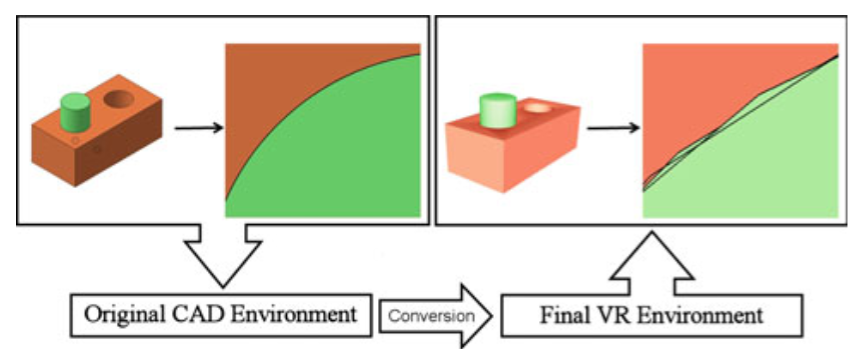
\includegraphics[keepaspectratio,width=0.6\linewidth]{CollisionDetection.png}
	\caption{Verlust der Genauigkeit bei der Konvertierung eines CAD-Models zu VR}
	\label{fig:LossOfAccuracy}
\end{figure}

\noindent VADE (\cite{noauthor_vade:_nodate}) ist eine virtuelle Assembly Design-Umgebung. In dieser werden je nach Situation die Freiheitsgrade der Bewegung des Bauteils eingeschränkt um das Zusammenbauen diverser Bauteile zu erleichtern. 
In der Abbildung \ref{fig:VADEAssembly} kann das Bauteil in der rechten Hand nur auf den hervorgehobenen Achsen bewegt werden. \\

\begin{figure}[h!]
	\centering
	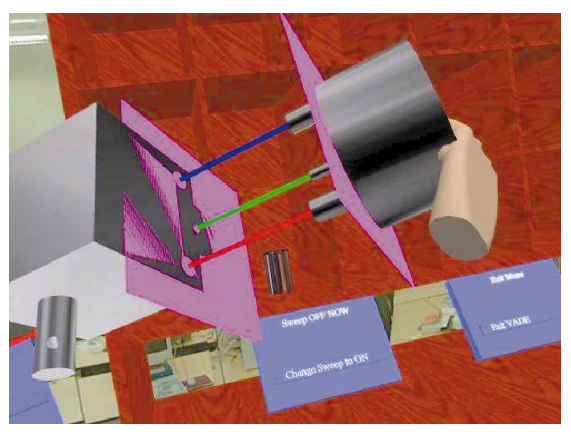
\includegraphics[keepaspectratio,width=0.5\linewidth]{VADE_PartsAssembly.png}
	\caption{Einschränkungen beim Zusammenbau in VADE}
	\label{fig:VADEAssembly}
\end{figure}

\noindent In der Arbeit "Virtual reality and augmented reality as a training tool for assembly tasks" (\cite{boud_virtual_1999}) wurde bereits 1999 untersucht ob das virtuelle Assembly Training einen Mehrwert gegenüber dem Training mit normalen Modellen in der realen Welt hat. Nach ihrer Aussage, hat das virtuelle Training Zukunft, da das Training bereits gestartet werden kann, ohne dass ein Prototyp vorhanden ist.

\section{Zusammenarbeit in der virtuellen Realität}
Für die Zusammenarbeit in der virtuellen Realität gibt es drei wesentliche Probleme welche in diversen Forschungen untersucht wurden (Collaborative User Interaction, User Representation und Communication Among People).

\subsection{Collaborative User Interaction}
Um eine gleichzeitige Interaktion am selben Objekt zu ermöglichen hat Márcio S. Pinho bereits 2002 (\cite{pinho_cooperative_2002}) eine Variante beschrieben, bei welcher die Freiheitsgrade der Benutzer separiert werden. Bei einem Würfel wäre das zum Beispiel wie folgt aufgeteilt. Ein Benutzer rotiert den Würfel während der andere Benutzer den Würfel in der virtuellen Welt bewegen kann. 
 
Berechne den Mittelwert aller Inputs der Nutzer. 
(Symmetric and Asymmetric Action Integration During Cooperative Object Manipulation in Virtual Environments)
 
Getrackte Objekte in der realen Welt, welche von den Nutzern manipuliert werden. (Einschränkungen) (Pyshare)
 
\subsection{User Representation}

Wie wird ein Benutzer einem anderen Benutzer in der virtuellen Realität dargestellt? 
Für viele Anwendungen reicht es den Kopf und die Hände des anderen Nutzers zu sehen.
3D-Körper gibt es in verschiedenen Variationen. Menschliche Körper besitzen mehrere hundert Muskeln und Gelenke. Sowas in VR umzusetzen ist schwierig.
Heutzutage gibt es Systeme, um das Gesicht und den Körper in der virtuellen Realität möglichst real zu animieren. Die Arbeit «Interactive Virtual Humans in Real-Time Virtual Environment» gibt eine gute Übersicht darüber. (Interactive Virtual Humans in Real-Time Virtual Environment)


\subsection{Communication Among people}

Kommunikation direkt via Audio-Aufnahmen integriert in die Applikation oder die Kommunikation mit der anderen Person direkt falls man sich im gleichen Raum befindet.
-	Synchrone oder asynchrone Kommunikation
Körpersprache wie zB. das Zeigen mit den Händen oder die Orientation des Kopfes


\chapter{Ideen und Konzepte}
\label{ch:Ideen_und_Konzepte}

\section{Single-User Prototyp}
Um dem Nutzer die Interaktion mit den Bauteilen so intuitiv und angenehm wie möglich zu machen, sind die folgenden Features in der Umsetzung geplant:

\subsection{Highlight}
\label{ch:highlight}
Um dem Benutzer zu zeigen, mit welchem Bauteil er interagieren kann, soll das Bauteil, in welchem sich seine Hand aktuell befindet, markiert werden. Dabei soll die Markierung für den Benutzer gut sichtbar sein, nicht aber die Sicht auf das Bauteil selbst versperren. \\
Im SteamVR-Asset befindet sich eine Beispiel Szene (Interactions\_Example), um die Handhabung mit dem Asset besser kennen zu lernen. In dieser Szene werden Objekte mit einer gelben Umrandung versehen, zu sehen in Abbildung \ref{fig:steamvr_highlight}, sobald sich ein Controller des Benutzers im Objekt befindet.

\begin{figure}[h!]
	\centering
	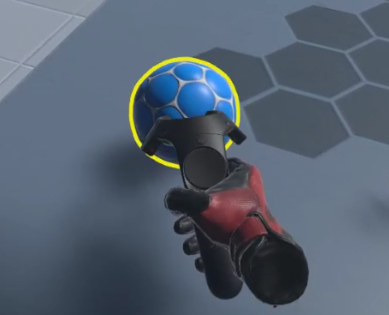
\includegraphics[keepaspectratio,width=0.4\linewidth]{img/SteamVR_Highlight.PNG}
	\caption{SteamVR Highlight}
	\label{fig:steamvr_highlight}
\end{figure}
	
\subsection{Snapping}
Bauteile in der virtuellen Realität präzise zu platzieren kann oft sehr schwierig sein. Um dem entgegenzuwirken sollen Bauteile, welche sich in der Nähe ihres vorgesehenen Ortes befinden, beim loslassen automatisch an ihre richtige Position bewegt werden. Um dem Benutzer mitzuteilen, dass das Bauteil an eine Position \grqq gesnappt\grqq{} werden kann, soll die Silhouette des Bauteils am vorgesehen Ort erscheinen. Um die Silhouette erscheinen zu lassen, könnte die gelbe Umrandung verwendet werden, welche im Kapitel \ref{ch:highlight} bereits erwähnt wurde. 
	
\subsection{Kollision}
\label{ch:kollision}
Beim Bewegen der Bauteile sollten diese mit anderen Bauteilen, welche sich in der virtuellen Umgebung befinden, kollidieren. Da alle Bauteile aber nur virtuell verfügbar sind und die Hand in der realen Welt nicht an etwas abprallen kann, muss dies in der virtuellen Realität simuliert werde. \\
Um dies zu Realisieren müssen beide Bauteile einen Collider besitzen. Sobald ein Kollisions-Event gesendet wird, wird das Bauteil von der Hand des Spielers losgelöst. Die Physik-Engine von Unity berechnet dann welche Auswirkungen die Kollision auf das Bauteil hat.
	
\subsection{Feedback beim Zusammenbau / Manipulation der Objekte}
\label{ch:feedback_zusammenbau_konzepte}
Da Bauteile nicht durch andere Bauteile hindurch bewegt werden können, muss dem Benutzer eine Art Feedback gegeben werden, sobald zwei Bauteile kollidieren. Dies soll dem Benutzer auch beim Zusammenbauen der Objekte behilflich sein. In der Tabelle \ref{tbl:varianten_zusammenbau} sind drei Varianten aufgelistet, welche dieses Problem lösen könnten. Anhand eines Nutzertests soll evaluiert werden, welcher dieser Varianten sich am besten für dieses Problem eignet.
	
\begin{center}
	\begin{tabularx} {\textwidth} { | B | B | B | }
		\hline
		\rowcolor{black}
		\color{white} \textbf{Variante} & \color{white} \textbf{Pro} & 
		\color{white} \textbf{Contra} \\
		\hline
		\vspace{1pt}
		Visuelles Feedback, falls ein Bauteil mit einem anderen kollidiert & 
		\begin{itemize} [leftmargin=*,noitemsep,topsep=0pt]
			\item Ist für alle Nutzer sichtbar
		\end{itemize} &
		\begin{itemize} [leftmargin=*,noitemsep,topsep=0pt]
			\item Kann dem Benutzer sehr unnatürlich erscheinen
		\end{itemize} \\
		\hline
		\vspace{1pt}
		Einschränkungen der Freiheitsgrade sobald das Bauteil eine gewisse Position erreicht, wie in Abbildung \ref{fig:VADEAssembly} zu sehen. 
		\vspace{2pt} & 
		\begin{itemize} [leftmargin=*,noitemsep,topsep=0pt]
			\item Das Zusammenbauen des Bauteils wird dem Benutzer erleichtert
		\end{itemize} &
		\begin{itemize} [leftmargin=*,noitemsep,topsep=0pt]
			\item Kein Feedback falls eine falsche Bewegung durchgeführt wird
		\end{itemize} \\
		\hline
		\vspace{1pt}
		Vibration Feedback bei einer falschen Bewegung & 
		\begin{itemize} [leftmargin=*,noitemsep,topsep=0pt]
			\item Der Benutzer bemerkt die falsche Bewegung, ohne hinzusehen
		\end{itemize} &
		\begin{itemize} [leftmargin=*,noitemsep,topsep=0pt]
			\item Nur der bearbeitende Benutzer bemerkt die falsche Bewegung
		\end{itemize} \\
		\hline	
	\end{tabularx}
\end{center}
\captionof{table}{Varianten für das Feedback beim Zusammenbau}\label{tbl:varianten_zusammenbau}

\subsection{Architektur}
% TODO: Architektur Diagramm

\pagebreak
\section{Multi-User Prototyp}
Der Multi-User Prototyp soll auf dem Single-User Prototyp aufbauen und alle Features von diesem implementieren. Die Erkenntnisse aus der ersten Nutzerevaluation sollen ebenfalls in den zweiten Prototypen einfliessen.

Anhand der Erkenntnissen aus den Recherchen, sind die folgenden Features in der Umsetzung geplant:

\subsection{Avatar-Repräsentation in der virtuellen Umgebung}
\label{ch:avatar-repraesentation}
Anhand der Recherchen, siehe Kapitel \ref{ch:avatar_repraesentation}, wurden folgende Varianten für eine Avatar-Repräsentation gefunden:
\begin{center}
	\begin{tabularx} {\textwidth} { | B | B | B | }
		\hline
		\rowcolor{black}
		\color{white} \textbf{Variante} & \color{white} \textbf{Pro} & 
		\color{white} \textbf{Contra} \\
		\hline
		\vspace{1pt}
		Kopf und Hände der Benutzer werden in der virtuellen Umgebung abgebildet & 
		\begin{itemize} [leftmargin=*,noitemsep,topsep=0pt]
			\item Gesten und Gaze können dargestellt werden
		\end{itemize} & 
		\begin{itemize} [leftmargin=*,noitemsep,topsep=0pt]
			\item Den Kopf und die Hände ohne Körper zu sehen kann sehr unnatürlich wirken
		\end{itemize} \\
		\hline
		\vspace{1pt}
		Einfacher Avatar welcher den Oberkörper abbildet & 
		\begin{itemize} [leftmargin=*,noitemsep,topsep=0pt]
			\item Funktioniert ohne zusätzliche Detektoren
		\end{itemize} & 
		\begin{itemize} [leftmargin=*,noitemsep,topsep=0pt]
			\item Versperrt dem andern Benutzer möglicherweise die Sicht auf Teile von relevanten Objekten
		\end{itemize} \\
		\hline
		\vspace{1pt}
		Ganzkörper Avatar & 
		\begin{itemize} [leftmargin=*,noitemsep,topsep=0pt]
			\item Ganzkörper Repräsentation des Gegenübers, erscheint daher natürlicher
		\end{itemize} & 
		\begin{itemize} [leftmargin=*,noitemsep,topsep=0pt]
			\item Schwer umzusetzen bezüglich des Trackings, da zusätzliche Detektoren verwendet werden müssen. Falls diese nicht richtig funktionieren erscheint der Avatar dem Gegenüber unnatürlich
		\end{itemize} \\
		\hline	
	\end{tabularx}
\end{center}
\captionof{table}{Varianten für die Avatar-Repräsentation}\label{tbl:varianten_avatar}

\bigskip
Für diesen Typ Applikation ist es nicht notwendig einen Ganzkörper Avatar zu verwenden. Dieser würde nur weitere Detektoren benötigen und bringt keinen Mehrwert. Die Gesten können auch mit einem einfachen Avatar dem Gegenüber gezeigt werden. \\
\noindent Ein einfacher Avatar bestehend aus Kopf, Oberkörper und den beiden Händen kann ohne zusätzlichen Detektoren umgesetzt werden. Dabei sehen die anderen Benutzer zusätzlich die Orientierung der anderen Benutzern, was für die Zusammenarbeit von Vorteil sein kann. Dementsprechend wird im Projekt ein Avatar mit einem Oberkörper verwendet.

\subsection{Kommunikation zwischen den Benutzern}
\label{ch:kommunikation_zwischen_benutzern}

\begin{center}
	\begin{tabularx} {\textwidth} { | B | B | B | }
		\hline
		\rowcolor{black}
		\color{white} \textbf{Variante} & \color{white} \textbf{Pro} & 
		\color{white} \textbf{Contra} \\
		\hline
		\vspace{1pt}
		Audio-Aufnahmen mit dem Mikrofon und Wiedergabe über die Kopfhörer des Gerätes & 
		\begin{itemize} [leftmargin=*,noitemsep,topsep=0pt]
			\item Kann über jegliche Distanzen verwendet werden
		\end{itemize} & 
		\begin{itemize} [leftmargin=*,noitemsep,topsep=0pt]
			\item Das Gerät muss ein Mikrofon sowie ein Lautsprecher besitzen
		\end{itemize} \\
		\hline
		\vspace{1pt}
		Direkte Kommunikation mit dem Gegenüber & 
		\begin{itemize} [leftmargin=*,noitemsep,topsep=0pt]
			\item Benötigt keine technische Implementation
		\end{itemize} & 
		\begin{itemize} [leftmargin=*,noitemsep,topsep=0pt]
			\item Beide Benutzer müssen sich im selben Raum befinden
		\end{itemize} \\
		\hline
		\vspace{1pt}
		Kommunikation anhand der Körpersprache - Gesten und Gaze & 
		\begin{itemize} [leftmargin=*,noitemsep,topsep=0pt]
			\item Einfach und verständlich
		\end{itemize} & 
		\begin{itemize} [leftmargin=*,noitemsep,topsep=0pt]
			\item Eingeschränkte Kommunikation
		\end{itemize} \\
		\hline	
	\end{tabularx}
\end{center}
\captionof{table}{Varianten für die Kommunikation zwischen den Benutzern}\label{tbl:varianten_kommunikation}

\bigskip
Da die Applikation auch verteilt über mehrere Standorte funktionieren soll, muss entweder Variante eins oder drei aus der Tabelle \ref{tbl:varianten_kommunikation} umgesetzt werden.  \\
Da die HTC Hive ein Mikrophon sowie Kopfhörer integriert hat, kann die erste Variante ohne zusätzliche Hardware umgesetzt werden. Um die Kommunikation zwischen den Benutzern so verständlich wie möglich zu machen wird zusätzlich zu der ersten Variante noch die dritte Variante umgesetzt, welche dank dem geplanten Avatar, beschrieben in Kapitel \ref{ch:avatar-repraesentation}, implementiert werden kann.


\subsection{Gleichzeitige Interaktion am selben Objekt}
Falls zwei Benutzer gleichzeitig dasselbe Objekt manipulieren wollen, muss eine Lösung gefunden werden, damit keine Inkonsistenzen zwischen den Benutzern entsteht, falls ein Benutzer das Bauteil an einen anderen Ort bewegt als der andere. Im Bereich der Gleichzeitigen Interaktion am selben Objekt gibt es sehr viele Varianten, über welche Forschungen und Paper veröffentlicht worden sind (siehe Kapitel \ref{ch:collaborative_user_interaction}). Anhand dieser wurde die nachfolgende Tabelle erstellt:

\begin{center}
	\begin{tabularx} {\textwidth} { | B | B | B | }
		\hline
		\rowcolor{black}
		\color{white} \textbf{Variante} & \color{white} \textbf{Pro} & 
		\color{white} \textbf{Contra} \\
		\hline
		\vspace{1pt}
		Separierung der Freiheitsgrade – Ein Nutzer steuert die Position, ein anderer die Rotation des Objektes &  &
		\begin{itemize} [leftmargin=*,noitemsep,topsep=0pt]
			\item Umständlich für eine Engineering Applikation
			\item Behindert die Zusammenarbeit
			\item Maximal zwei Benutzer
		\end{itemize} \\
		\hline
		\vspace{1pt}
		Berechnung des Mittelwerts aller Inputs der Nutzer & 
		\begin{itemize} [leftmargin=*,noitemsep,topsep=0pt]
			\item Gleichzeitige Manipulation
		\end{itemize} & 
		\begin{itemize} [leftmargin=*,noitemsep,topsep=0pt]
			\item Das Manipulierte Objekt verhält sich nicht natürlich und zerstört so die Immersion
		\end{itemize} \\
		\hline
		\vspace{1pt}
		Abstrahierte Objekte in der realen Welt & 
		\begin{itemize} [leftmargin=*,noitemsep,topsep=0pt]
			\item Natürliches Verhalten
			\item Natürliches Feedback bei der Manipulation
		\end{itemize} & 
		\begin{itemize} [leftmargin=*,noitemsep,topsep=0pt]
			\item Benutzer müssen sich im selben Raum befinden
			\item Objekt und Hände müssen getracked werden
		\end{itemize} \\
		\hline
		\vspace{1pt}
		Zauberstab – Nur der Benutzer mit dem Zauberstab kann das Objekt manipulieren &
		\begin{itemize} [leftmargin=*,noitemsep,topsep=0pt]
			\item Natürliches Verhalten, da nur ein Nutzer das Objekt manipuliert
		\end{itemize} &
		\begin{itemize} [leftmargin=*,noitemsep,topsep=0pt]
			\item Nur ein Benutzer kann die Umgebung bearbeiten
		\end{itemize} \\
		\hline	
		\vspace{1pt}
		«First come, First grab» Der Benutzer welcher eine Interaktion als erstes beginnt hat so lange die Macht über das Objekt bis er dieses wieder loslässt. & 
		\begin{itemize} [leftmargin=*,noitemsep,topsep=0pt]
			\item Natürliches Verhalten, da nur ein Nutzer das Objekt manipuliert
		\end{itemize} &
		\begin{itemize} [leftmargin=*,noitemsep,topsep=0pt]
			\item Nur ein Benutzer kann das Objekt bearbeiten
			\item Andere Benutzer müssen sehen, ob sie das Objekt aktuell manipulieren können oder nicht
		\end{itemize} \\
		\hline	
	\end{tabularx}
\end{center}
\captionof{table}{Varianten für gleichzeitige Interaktion am selben Objekt}\label{tbl:varianten_gleichzeitige_interaktion}

\bigskip
Die erste Variante macht in der umzusetzende Applikation die Zusammenarbeit umständlicher als es sein muss. Da ein Objekt oftmals nicht nur die Position ändern soll sondern auch die Rotation müssten bei den meisten Interaktionen mehrere Benutzer beteiligt sein. \\
Die Variante bei welcher der Mittelwert aller Inputs genommen wird, wird ebenfalls nicht umgesetzt, da sich die Bewegung des Objektes für alle beteiligten Benutzer unnatürlich anfühlen würde. \\
Die Variante mit den abstrahierten Objekte in der realen Welt würden den Benutzern das natürlichste Verhalten geben, kann aber nicht umgesetzt werden, da die Applikation auch verteilt funktionieren soll und sich die Benutzer für diese Variante im selben Raum befinden müssten. \\
Dementsprechend werden die letzten beiden Varianten implementiert und anhand von Nutzertests evaluiert, welche Variante sich für diese Applikation besser eigenen würde.

\subsection{Architektur}

\chapter{Methode}

\section{Projektinformationen}

\subsection{Vorgehensmodell}

Alle Wirtschaftsprojekte an der Hochschule Luzern fallen in eine der folgenden Kategorien:

\begin{enumerate}
	\item Einsatz von Standardsoftware und Services
	\item Software- und Produktentwicklung
	\item Innovationsprojekt
	\item IT-Infrastrukturentwicklung
	\item Strukturierte Analyse und Konzeption von Systemen und Abläufen
\end{enumerate}

Dabei ist dieses Projekt als Innovationsprojekt und Softwareentwicklung klassifiziert worden. Wir erwarteten daher unter anderem, eine Evaluation, Recherchen und weitere Unbekannten. Um auf diese eingehen zu können, entschied sich das Team dafür die hybride, inkrementelle Agile Methode zu verwenden.

\subsection{Agile Projektmethode}

Die agile Projektmethode zielt darauf ab in einem ungewissen und sich verändernden Umfeld zu bestehen. Insbesondere bedeutet dies, das auf sich verändernde Voraussetzungen schnell reagiert werden kann und dabei ein funktionierendes Produkt entsteht \parencite{AgileAlliance2015}. Dies soll durch eine enge Zusammenarbeit mit dem Auftraggeber und guter teaminterner Kommunikation erreicht werden.

\parencite{BaumannWicki2018}

\subsection{Ermittlung offener Projektrahmenbedingungen}
\label{ch:evaluation}

\subsection{Projektanforderungen}
Mittels einer Machbarkeitsstudie und einem Proof of Concept soll untersucht werden ob es möglich ist bis zu 120 \gls{RFID} Tags in einem Behälter mit der Dimension 600x400x320mm zu identifizieren.

\begin{itemize}
	\item Es sollen mindestens zwei Lösungskonzepte für eine als Auswahl der Machbarkeitsstudie entwickelt werden.
	\item Die Lösungskonzepte müssen auf deren technische Realisierbarkeit untersucht werden.
	\item Es muss mindestens ein entwickeltes Konzept für die Machbarkeitsstudie verwendet werden.
	\item Die Machbarkeitsstudie muss eine Kostenrechnung für die Lösungsansätze beinhalten.
	\item Es soll eine MVP entwickelt werden, welches vom Kunde verwendet werden kann.
\end{itemize}

\subsubsection{Anforderungen an Lösungsansätze, Proof of Concept und MVP}

\begin{itemize}
	\item Die Lösungskonzepte müssen mit dem Lagersystem kommunizieren können
	\item Die Lösungskonzepte müssen die \gls{RFID} Tags in weniger als 1 Sekunden identifizieren können.
	\item Die Lösungskonzepte müssen für das bestehende Hochregallager der Speicherbibliothek verwendbar sein.
	
	\item Das Proof of Concept muss technisch aufzeigen, wie viele \gls{RFID} Tags in einer Sekunde gelesen werden können.
	\item Das Proof of Concept soll eine \gls{RFID} Lesezuverlässigkeit von 95\% aufweisen.
	
	\item Das MVP soll mit der Datenbank des Lagersystems kommunizieren können.
	\item Das MVP soll in einem von Störfaktoren bereinigten Zustand die gleiche Anzahl \gls{RFID} Tags lesen können wie im Proof of Concept definiert.
	\item Das MVP soll erkennen, wenn eine Box ein Exemplar enthält, welches nicht dieser Box zugehörig ist und dies als eine Unstimmigkeit markieren.
	\item Das MVP soll in der Lage sein, dem Endbenutzer in beliebiger Form mitzuteilen, welcher Behälter eine Unstimmigkeit enthält.
\end{itemize}

\subsection{Einschränkungen und Abgrenzungen}

\section{Machbarkeitsstudie}


\chapter{Realisierung}

\newpage
-\section{Systemspezifikation}
\label{sec:SysSpec}

\subsection{Anforderungen}
\label{ch:Anforderungen}

\subsection{Kontext}

\subsection{Komponentendesign}

\subsection{Architektur \& Design}

\subsection{Interne Schnittstellen}

\subsection{Klassendiagramm}

\subsection{Anforderungen der Software}

\subsection{Umsetzung Programmierung}

\subsection{Testing}


\chapter{Projektmanagementplan}

\section{Projektorganisation}

\vspace{1em}

\begin{tabularx}{\textwidth}{|X|X|}
	\hline
	\textbf{Projektbeteiligte} & \textbf{Funktionen} \\
	\hline
	Mike Märki & Stakeholder/Auftraggeber \\
	\hline
	Martin Jud & BDA Experte \\
	\hline
	Pascal Baumann & Product Owner \& Dev Team \\
	\hline
	Dane Wicki & Scrum Master \& Dev Team \\
	\hline
\end{tabularx}

\subsection{Organigramm}
\begin{figure}[h!]
	\centering
	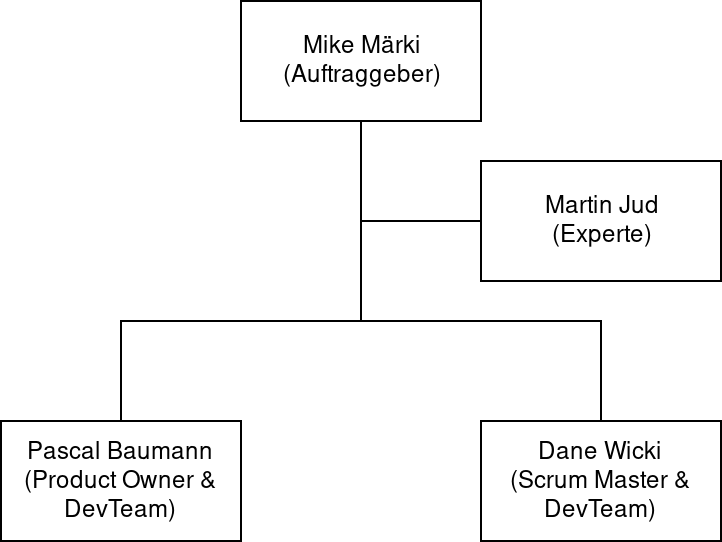
\includegraphics[keepaspectratio, width=0.6\textwidth]{OrganigrammBDA_BAWI.png}
\end{figure}


\section{Rahmenplan}
\subsection{Meilensteine}
\label{ssec:Meilensteine}
Für das Projekt wurden vier Meilensteine definiert, welche jeweils im Vierwochenzyklus auftreten. Diese Meilensteine sind in Abbildung \ref{fig:Milestones} dargestellt.

\begin{figure}[h!]
	\centering
	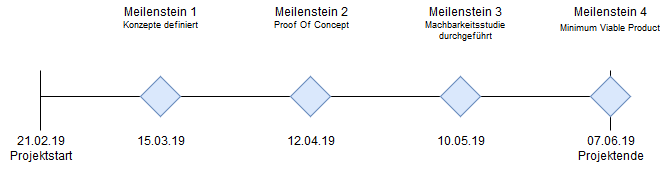
\includegraphics[keepaspectratio,width=0.8\linewidth]{Milestones.png}
	\caption{Die für das Projekt definierten Meilensteine}
	\label{fig:Milestones}
\end{figure}

\subsection{Grobplan}

Aus den im Kapitel \ref{ssec:Meilensteine} definierten Meilensteine wurden acht Sprints von zwei Wochen abgeleitet. In diesen werden sowohl die Artefakte wie Projektdokumentation, Machbarkeitsstudien und Systemspezifikation, wie auch das Produkt entwickelt. Der grobe Rahmenplan ist in Abbildung \ref{fig:Rahmenplan_1} dargestellt.

\begin{figure}[h!]
	\centering
	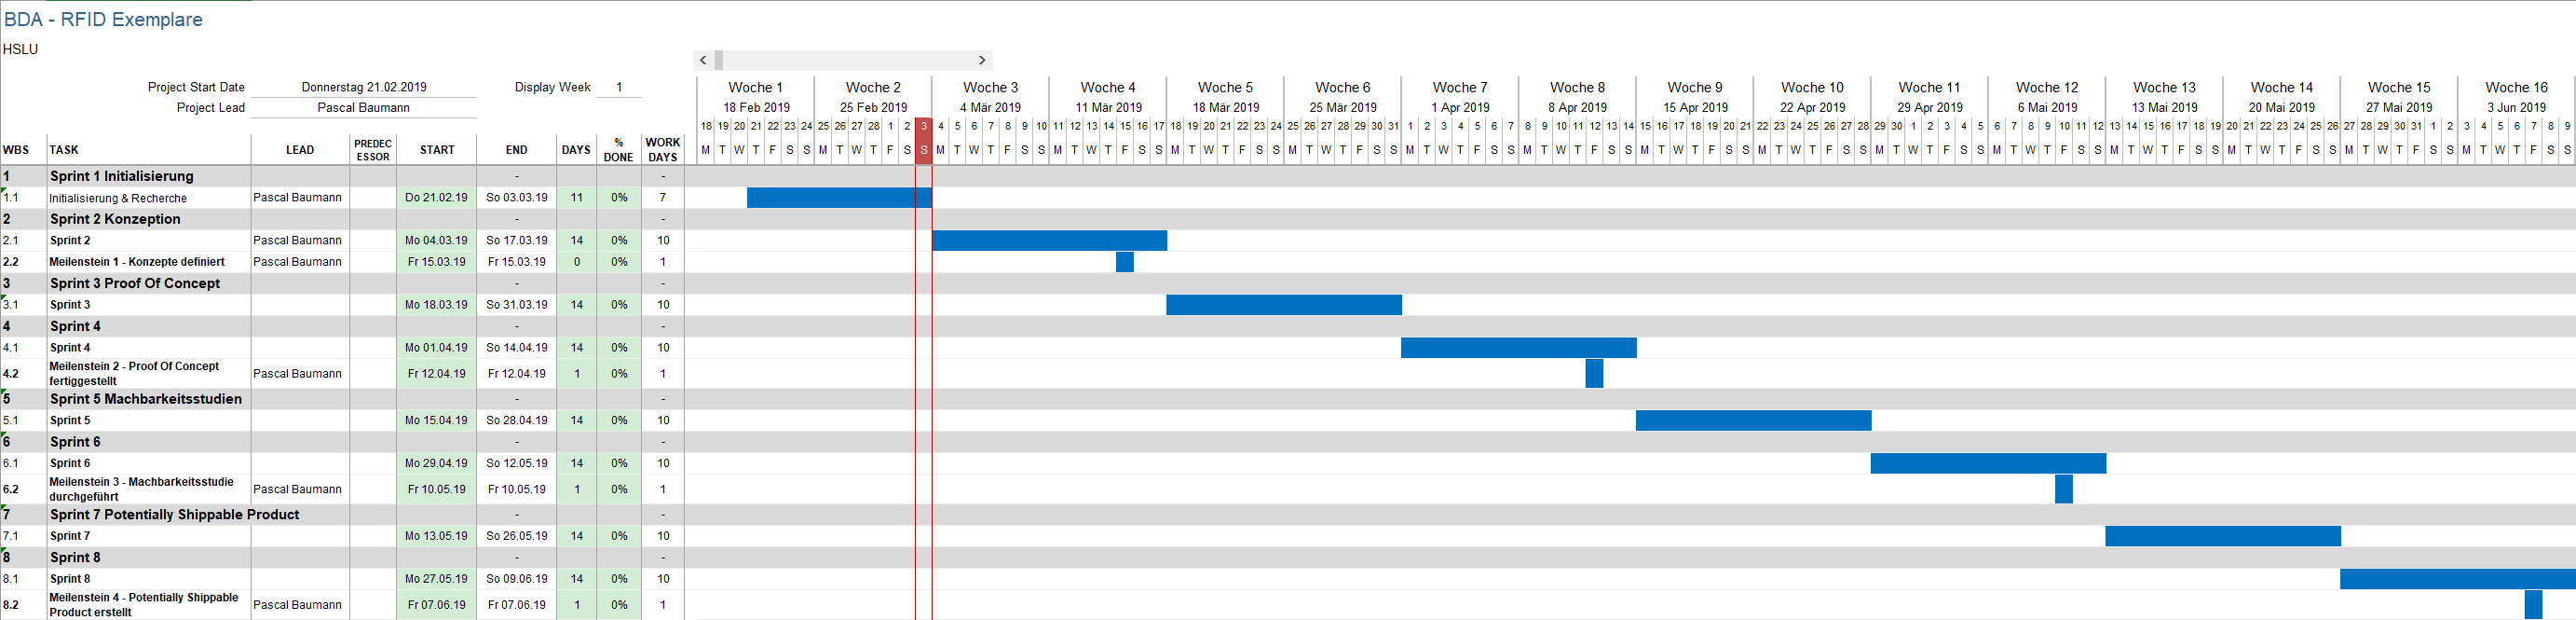
\includegraphics[keepaspectratio,width=\linewidth]{Grobplan.png}
	\caption{Übersicht der Sprints im Rahmenplan}
	\label{fig:Rahmenplan_1}
\end{figure}

\newpage

\section{Tools}
\label{sec:Tools}

\subsection{Versions Kontrolle}
\begin{table}[h!]
	\begin{tabular}{p{0.5\textwidth} p{0.5\textwidth}}
		\hline
		\textbf{Tool} & \textbf{Version} \\
		\hline
		GitKraken & 4.2.2 \\
		\hline
		git & 2.21.0 \\
		\hline
		GitHub & GitHub.com \\
		\hline
	\end{tabular}
	\caption{Verwendete Versionen der Versionierungssysteme}
\end{table}

\subsection{Dokumentation}
\begin{table}[h!]
	\begin{tabular}{p{0.5\textwidth} p{0.5\textwidth}}
		\hline
		\textbf{Tool} & \textbf{Version} \\
		\hline
		TeX Live & 2018 \\
		\hline
		MiKTex & 2.9.6637 \\
		\hline
		Mendeley Desktop & 1.19.2 \\
		\hline
		MS Excel & 16.0.11231.20164 \\
		\hline
	\end{tabular}
	\caption{Verwendete Versionen der Hilfsmittel für die Dokumentation}
\end{table}


\subsection{Repositories \& Buildtools}
\begin{table}[h!]
	\begin{tabular}{p{0.5\textwidth} p{0.5\textwidth}}
		\hline
		\textbf{Name} & \textbf{URL} \\
		\hline
		Dokumentation & \url{https://github.com/HSLU-BaumannWicki/BDA_FS19-Dokumentation} \\
		\hline	
		Travis CI &  \url{https://travis-ci.org/HSLU-BaumannWicki/BDA_FS19-Dokumentation} \\
		\hline
	\end{tabular}
	\caption{Verwendete Repositories}
\end{table}

\subsection{Übrige}
\begin{table}[h!]
	\begin{tabular}{p{0.5\textwidth} p{0.5\textwidth}}
		\hline
		\textbf{Tool} & \textbf{Verwendung} \\
		\hline
		Trello & Aufgabenverwaltung \\
		\hline
		WhatsApp & Kommunikation im Team \\
		\hline
		OneDrive Online & Dokumentenspeicher \\
		\hline	
	\end{tabular}
	\caption{Übrige Hilfsmittel}
\end{table}

\clearpage

\section{Risikomanagement}

Es werden mögliche Risiken, welche während dem Projekt auftreten können aufgezählt. Diese werden auf Eintrittswahrscheinlichkeit und Schadensmass eingeschätzt, danach wird entschieden, welche Massnahmen getroffen werden können, und was deren Auswirkungen sind.

\subsection{Definitionen}
\label{sssec:Def}
\vspace{1em}
\noindent
Eintrittswahrscheinlichkeit:

\vspace{1em}
\noindent
\begin{tabularx}{\textwidth}{|l|l|X|}
	\hline
	\textbf{Stufe} & \textbf{Bezeichnung} & \textbf{Beschreibung} \\
	\hline
	1 & unvorstellbar & Möglich aber eher unwahrscheinlich. Tritt nie oder einmal in 16 Wochen auf \\
	\hline
	2 & unwahrscheinlich & Kann in 16 Wochen kein oder ein Mal eintreten\\
	\hline
	3 & vorstellbar & Kann in 16 Wochen ein bis zwei Mal eintreten \\
	\hline
	4 & wahrscheinlich & Kann in 16 Wochen bis zu drei Mal eintreten \\
	\hline
	5 & häufig & Kann in 16 Wochen sieben Mal eintreten\\
	\hline
\end{tabularx}

\vspace{1em}
\noindent
Schadensausmass:

\vspace{1em}
\noindent
\begin{tabularx}{\textwidth}{|l|l|X|}
	\hline
	\textbf{Stufe} & \textbf{Bezeichnung} & \textbf{Beschreibung} \\
	\hline
	1 & unwesentlich & Die Aufgabenerfüllung wird höchstens geringfügig beeinträchtigt, finanzieller Schaden ist im Rahmen des Projekts nicht beeinflussend. Personenschäden treten nicht auf. \\
	\hline
	2 & geringfügig & Wahrnehmbare Gefährdung / Einfluss auf das Projekt. Personenschäden treten nicht auf. \\
	\hline
	3 & mittelmässig & Wahrnehmbare Gefährdung / Einfluss auf das Projekt. Verzögerungen zur Folge. Finanzieller Schaden strapaziert das Projektbudget. Personenschäden treten nicht auf. \\
	\hline
	4 & kritisch & Starke Gefährdung des Projekts. Extreme Verzögerungen zur Folge. Finanzieller Schaden übersteigt das Projektbudget. Personenschäden treten geringfügig auf.\\
	\hline
	5 & katastrophal & Projektabbruch zur Folge. Finanzieller Schaden kann zum Projektstopp führen. Verletzung der Persönlichkeitsrechte. \\
	\hline
\end{tabularx}

\newpage

\subsection{Risikokatalog}
\label{sssec:Risikokatalog}
Legende:
\begin{itemize}
	\item \textbf{S}chadensausmass bei Eintreffen des Risikos
	\item \textbf{W}ahrscheinlichkeit das Risiko eintrifft
	\item \textbf{K}ategorie: \textbf{T}echnisches oder \textbf{P}rojektbezogenes Risiko
	\item \textbf{A}uswirkung auf das Projekt. Produkt aus S und W
\end{itemize}

\vspace{1em}
\noindent
\begin{table}[htb]
	\begin{tabularx}{\textwidth}{|l|X|l|l|l||l|}
		\hline
		\textbf{Nr.} & \textbf{Beschreibung / Risiko} & \textbf{K} & \textbf{S} & \textbf{W} & \textbf{A} \\
		\hline
		1 & Meilensteine werden nicht erreicht & P & 4 & 2 & 8 \\
		\hline
		2 & Teammitglied fällt aus & P & 4 & 1 & 4 \\
		\hline
		3 & Fehlkommunikation im Team & P & 4 & 1 & 4 \\
		\hline
		4 & Produkt entspricht nicht den Kundenanforderungen & P & 5 & 2 & 10 \\
		\hline
		5 & Umsetzung des Produkts technisch nicht möglich & T & 4 & 3 & 12 \\
		\hline
		6 & Datenverlust & T & 5 & 2 & 10 \\
		\hline
		7 & Lieferschwierigkeiten von Teilen & P & 3 & 3 & 9 \\
		\hline
	\end{tabularx}
	\caption{Die im Projekt identifizierten Risiken}
	\label{tbl:Risks}
\end{table}

\vspace{1em}

\begin{figure}[h!]
	\centering
	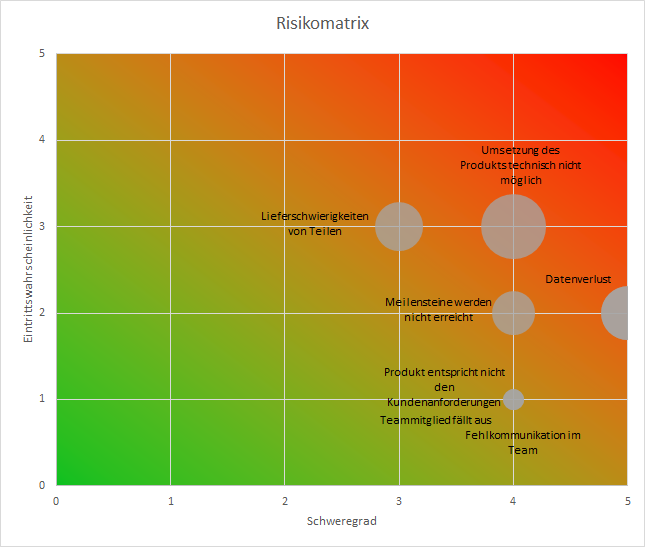
\includegraphics[keepaspectratio, width=0.6\textwidth]{Risks_before.png}
	\caption{Auswirkungen der in Tabelle \ref{tbl:Risks} identifizierten Risiken}
\end{figure}

\newpage

\subsubsection{Massnahmen}

\begin{table}[htb]
	\begin{tabularx}{\textwidth}{|l|X|}
		\hline
		\textbf{Nr.} & \textbf{Beschreibung Massnahme} \\
		\hline
		1 & Meilensteine werden in zwei Zweiwöchigen Sprints absolviert. Die Tasks pro Sprint werden weiter detailliert heruntergebrochen. So sollen die Arbeiten sowohl auf Makro- wie Mikrosicht eingeplant werden. \\
		\hline
		2 & Arbeiten werden so strukturiert und dokumentiert, dass das zweite Mitglied diese auch übernehmen kann. Es werden Spezialisierungen der Teammitglieder insoweit verhindert, dass Wissenslücken minimiert werden. Recherchen sollen Zusammenfassungen und Merkblätter über die gewonnenen Erkenntnisse als Resultat haben.\\
		\hline
		3 & Der Kontakt wird von beiden Teammitgliedern sowohl horizontal im Team wie auch vertikal zu den Stakeholdern aktiv gesucht. Es werden den Arbeiten auch teambildende Aktivitäten zusammen absolviert.\\
		\hline
		4 & Der Kunde muss den Fortschritt alle vier Wochen in einer Sitzung kontrollieren, avisieren und, wenn nötig, Anpassungen fordern.\\
		\hline
		5 & Es soll während den Recherchen schon im Hinblick auf die technische Umsetzung acht gegeben werden.\\
		\hline
		6 & Sowohl produzierten Artefakte, wie auch aktuelle getätigte Arbeiten werden auf auswärtige Plattformen ausgelagert.\\
		\hline
		7 & Teile werden bei Bedarf sofort bestellt, es werden inländische, etablierte Lieferanten, vor evtl. günstigeren Ausländischen vorgezogen.\\
		\hline
	\end{tabularx}
	\caption{Massnahmen um Effekte oder Eintrittswahrscheinlichkeit zu reduzieren}
\end{table}

\vspace{1em}

\begin{table}[htb]
	\begin{tabularx}{\textwidth}{|l|X|l|l|l||l|}
		\hline
		\textbf{Nr.} & \textbf{Beschreibung / Risiko} & \textbf{K} & \textbf{S} & \textbf{W} & \textbf{A} \\
		\hline
		1 & Meilensteine werden nicht erreicht & P & 4 & 1 & 4 \\
		\hline
		2 & Teammitglied fällt aus & P & 3 & 1 & 3 \\
		\hline
		3 & Fehlkommunikation im Team & P & 4 & 1 & 4 \\
		\hline
		4 & Produkt entspricht nicht den Kundenanforderungen & P & 5 & 1 & 5 \\
		\hline
		5 & Umsetzung des Produkts technisch nicht möglich & T & 4 & 3 & 12 \\
		\hline
		6 & Datenverlust & T & 5 & 1 & 5 \\
		\hline
		7 & Lieferschwierigkeiten von Teilen & P & 3 & 2 & 6 \\
		\hline
	\end{tabularx}
	\caption{Neueinschätzung der Risiken nach Einführung der Massnahmen}
	\label{tbl:Massnahmen}
\end{table}

\vspace{1em}

\begin{figure}[h!]
	\centering
	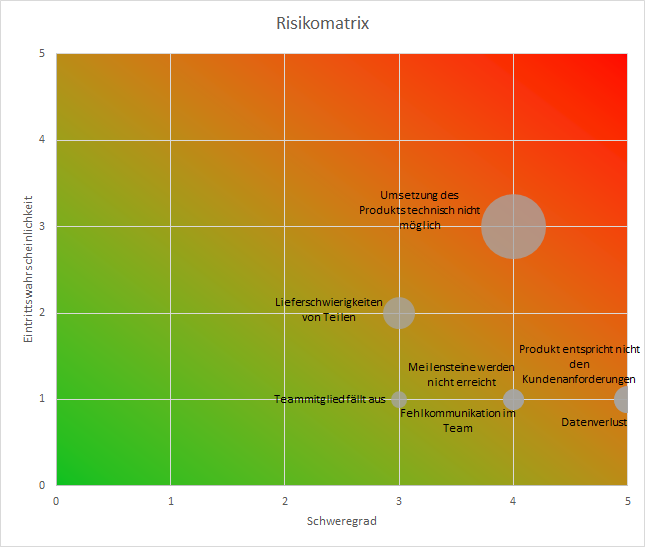
\includegraphics[keepaspectratio, width=0.6\textwidth]{Risks_after.png}
	\caption{Auswirkungen der Risiken nach den in Tabelle \ref{tbl:Massnahmen} vorgeschlagenen Massnahmen}
\end{figure}


\chapter{Evaluation und Validation}
\label{ch:Eval}

\section{Vergleich mit Anforderungen}
\label{sec:VergleichAnforderungen}

\chapter{Ausblick}
\label{ch:Ausblick}

Mit den vorliegenden Prototypen wurde eine solide Grundlage für das gemeinsame Arbeiten in der virtuellen Realität geschaffen. In einem weiteren Schritt würden nun die Erkenntnisse aus der zweiten Nutzerevaluation in die Applikation eingebracht und die folgenden zwei Anpassungen gemacht:

\begin{itemize}
	\item Im zweiten Teil des Projektes wurde aus zeitlichen Gründen nur die Vibrations-Rückmeldung umgesetzt. Anhand der Rückmeldungen der ersten Nutzerevaluation würden diverse Teilnehmer eine Kombination dieser Variante mit der Variante bevorzugen, bei welcher die Freiheitsgrade eingeschränkt werden. Um bei einer Maschine zum Beispiel eine Schraube einzusetzen, würde die Kombination dieser beiden Variante eine grosse Hilfe sein.
	
	\item Damit eine neue Maschine in der Applikation integriert werden kann sind aktuell viele Schritte notwendig. Um dies zu erleichtern müsste die Integration entweder automatisiert oder die Anzahl Schritte erheblich verringert werden. Zudem können zum aktuellen Zeitpunkt nur Modelle implementiert werden, bei welchen jedes Bauteil eine Rotation von 0$^{\circ}$ auf allen Achsen hat. Ansonsten funktioniert das «Snapping» nicht richtig.
\end{itemize}


\newpage

\pagenumbering{Roman}

\appendix

\printglossary

\listoffigures

\listoftables

\listofmyequations \pagebreak

\printbibliography

\end{document}
